\documentclass[a4paper,11pt]{article}
\usepackage[utf8x]{inputenc}
\usepackage[T1]{fontenc}
\usepackage[francais]{babel}
\usepackage{amsmath,amssymb}
\usepackage{fullpage}
\usepackage{xspace}
\usepackage{verbatim}
\usepackage{graphicx}
\usepackage{listings}
\usepackage{stmaryrd}
\usepackage[usenames,dvipsnames]{color}
\usepackage{url}
\usepackage{caption}


\title{Compte-rendu du projet d'algorithmique}
\author{Michaël Bleuez \and Clément Malleret}
\date{Mai 2019}



\begin{document}

\maketitle

Index
\begin{enumerate}
    \item {Résumé}
    \item {Etymologie}
    \item {Présentation des différents algorithmes}
    \item {Choix du meilleur algorithme}
    \item {Performances}
    \item {Evolution de l'algorithme}
    \item {Possibilités d'améliorations}
    \item {Conclusion}
\end{enumerate}

\section{Résumé}
Le problème posé est de rassembler les points d'une liste en "composantes connexes" en considérant que  deux points sont "connexes" si ils sont à moins de $distance$ (notée $d$) l'un de l'autre.
\smallbreak
L'algorithme que nous proposons peut prendre en entrée une liste de points de coordonnées quelquonques (non limitées à $[0,1]$, et pas forcément aléatoires) \textbf{en dimension quelquonque}.
\smallbreak
Sa complexité en temps est au pire $\mathcal{O}(n \log(n) a^k)$ où $n$ est la longueur de la liste de points, $a \sim 2.2$ et $k$ est la dimension de l'espace contenant les points. L'effet de $d$ sur la complexité est important mais reste borné, c'est pourquoi on ne le représente pas (il aussi dépend d'autres facteurs, tels que le nombre de points, la dimension de l'espace et les coordonnées maximum/mimimun des points).




\section{Etymologie}
\begin{enumerate}
    \item {Densité (d'une distribution de points): notion fondamentale. Traduit le fait que les points sont rassemblé en composantes +/- grosses par rapport à leur nombre. Plus la distribution est dense plus les composantes connexes rassemblent de points. En dimension 2, la densité est proportionnelle à $d * \sqrt{n}$}
    \item{Cluster: classe d'objets qui forment les composantes connexes découvertes et s'agrandissant au fur à mesure. Se fusionnent au sens ensembliste usuel, de plus chaque point réference son cluster et chaque cluster réference ses points}
    \item {Quadrant: classe d'objets qui forment une 'boite' dans l'espace (dimension quelquonque). Ils forment un arbre où les quadrants enfants sont géométriquement à l'intérieur de leur parent.}
\end{enumerate}














\section{Présentation des différents algorithmes}

Nous avons mis au point 3$^{(*)}$ différents algorithmes afin de répondre au problème posé. Ils visent chacun à être efficaces pour certains cas, et sont complémentaires les uns des autres.\\


Les deux premiers se basent sur la représentation de l'espace par un quadrillage, et sont efficaces pour des distributions 2D uniformes,  tandis que le dernier s'appuie sur le principe de R-tree et marche dans toutes les situations.
    \bigbreak
    \bigbreak
    * 6 si on compte les cas "spéciaux"
    \bigbreak

\subsection{Algorithme "standard" : quadrillage de maille $d$ ou plus si affinités}
	\paragraph{Fonctionnement (nota bene: uniquement en dimension 2)}
	\begin{enumerate}
		\item \textbf{Pré-traitement des données} \\
			On représente le plan par un quadrillage, dont les cases (carrées) ont un côté de distance $d$ ou plus (si d est exagérement petite, on ira jusqu'à l'ignorer et prendre des cases de taille $\dfrac{1}{\sqrt{n}}$), distance qu'on appellera $c$ (pour côté). $c$ ($=\frac{f}{d}$) est calculé à partir d'un facteur $f$ de densité (presque) proportionnel a $d \times \sqrt{n}$, où $n$ est le nombre total de points. (Ce facteur est d'origine statistique, le "presque" ainsi que les différents niveaux de densité 'limites' ont un lien avec la théorie de la percolation).
			\smallbreak
			Plus la distribution a une faible densité (en pratique $d$ est petit), plus $f$ sera grand pour compenser. \\
Les composantes sont représentées par une classe $cluster$, qui comporte un ID, une liste de points contenus et.\\
L'algorithme, dans un premier temps, crée le quadrillage et place les points dans la case à laquelle ils appartiennent. Cette opération se fait en $\mathcal{O}(n)$, car on peut calculer les coordonnées de la case à laquelle appartient un point à partir des coordonnées de ce dernier.\\
		\item \textbf{Parcours de la grille} \\
		On parcourt ensuite le quadrillage case par case. Pour chacune des cases, on regarde celle-ci et les cases adjacentes, et on énumère les combinaisons de points appartenant à ces cases. Si la distance entre 2 points est inférieur à $d$, on fusionne leurs clusters.\\
On ne parcours pas tous les voisins : en effet, l'opération d'énumération des points de 2 cases est symétrique : on ne parcours pas les couples de cases précédemment parcourues.\\
        \item \textbf{Calcul des tailles des composantes} \\
On re-parcours finalement tous les points, et si sa composante n'a pas déjà été parcourue, on ajoute sa taille à la liste à renvoyer.
\smallbreak
Le principe de calcul des tailles de composantes est le même pour tous les algorithmes
	\end{enumerate}
		



\paragraph{Meilleur/Pire des cas} \mbox{} \\
Ici, le \textbf{pire des cas} est si tous les points sont contenus dans la même case, auquel cas on énumère toutes les combinaisons de points possibles : l'algo est alors en $\mathcal{O}(n^2)$. Cet algo est donc inefficace dans le cas ou les cases (qui ne peuvent pas être de coté $c < d$) sont grandes et contiennent beaucoup de points.\\
Cependant, il est \textbf{optimal} dans le cas de points peu denses : dans le cas où il y aurait en moyenne 1 ou 2 points par case, sa complexité est en $\mathcal{O}(\Sigma$(nombre-de-points-par-case)²$)$, et dépend donc énormément de la manière dont les points sont distribués.   \\
\textbf{En pratique,} à partir d'une série de tests, on détermine que la compléxité temporelle est en $\mathcal{O}(n\log n)$ pour des entrées moyennement ou peu denses.\\
On utilisera donc cet algorithme dans le cas de \textbf{distribution peu denses}.

\subsection{Algorithme "sqrt2" : quadrillage de taille $\dfrac{d}{\sqrt{2}}$}
	\paragraph{Fonctionnement (uniquement en dimension 2)}
	\begin{enumerate}
		\item \textbf{Rassemblement en composontantes connexes} \\
		On représente de nouveau le plan comme un quadrillage, mais cette fois-ci, $c$ est fixe, de valeur $\dfrac{d}{\sqrt{2}}$. L'intérêt d'une telle valeur est que tous points contenus dans une même case sont forcément dans la même composante connexe.\\
		Compte-tenu de ceci, on va modifier la façon dont le quadrillage fonctionne : on utilise toujours une classe $cluster$, mais elle est associée cette fois-ci non pas à des points, mais à des cases.\\
		On commence donc par construire le quadrillage, opération qui comme précédemment est en $\mathcal{O}(n)$.
		
	 \item \textbf{Calcul des composantes} \\
	 	Le calcul des composantes est assez similaire : Pour chaque case, on énumère les combinaisons de points entre la case elle-même est ses voisines "étendues" : en effet, avec $c < d$, il faut regarder plus loin que les voisins directs pour ne pas rater de composantes.\\
	 	Lorsque la distance entre deux points de deux cases voisines est inférieure à $d$, on fusionne alors les deux $Clusters$ de leurs cases.\\
	 	Puis, pour finir, on construit la liste des tailles des composantes de la même façon que pour l'algorithme précédent : opération qui se fait en $\mathcal{O}(n)$.
	
	\end{enumerate}
\paragraph{Meilleur/Pire des cas} \mbox{} \\
Ici, le \textbf{meilleur des cas} est si tous les points sont contenus dans la même case : on construit alors directement dans le pré-traitement la composante en $\mathcal{O}(n)$.\\
Le \textbf{pire des cas} est quand les points sont peu denses (la distance $d$ est petite) : on se retrouve alors avec beaucoup de cases contenant juste un point ; or comme on parcourt toutes les cases non-vides, et que celles-ci sont petites et nombreuses, l'algorithme voit sa complexité augmenter.\\
\textbf{En pratique,} on constate que pour des distributions de points denses, on a une complexité (en moyenne) en $\mathcal{O}(n)$.\\
Cet algorithme complète très bien le précédent : leurs meilleurs et pires des cas sont opposés. On utilisera celui-ci pour les \textbf{entrées denses}.\\

\subsection{Algorithme "not-random" : R-tree}
    \paragraph{Fonctionnement (marche en dimension quelquonque)}
    \begin{enumerate}
        \item \textbf{Qui dit tree dit arbre}\\
        L'arbre ici implementé est de principe de fonctionnement similaire à un r-tree,
        plus quelques subtilités bien utiles. Dans la suite il sera important de remarquer que l'arbre que l'on construit est volontairement déséquilibré. Les noeuds de l'arbre sont les objets de la classe Quadrant et comportent plusieurs attributs supplémentaires, notamment: list-point-inside, leafs (est une feuille), dense (contient beaucoup de points et est traité différement).
        \item \textbf{Diviser}\\
        C'est simple de diviser une ligne (quadrant en dimension 1) en deux, et presque aussi simple de diviser un rectangle en quatre. Lors de la création de l'arbre, on divise un quadrant/noeud parent de dimension \textbf{quelquonque} (ce qui est beaucoup plus dur).
        \smallbreak
        Concrètement, on crée 2,ou 4, ou 8 etc.. $(2^{dimension})$ quadrants fils qui remplissent géométriquement le quadrant parent.
        \smallbreak
        On arrête la récursion lorsque soit le quadrant parent est presque vide ou de trop petite taille. (!!si il est petit mais contient encore beaucoup de points on passe mode "dense" et le principe change).
	Chaque quadrant fils est équipé à sa naissance d'un double agrandi de d de sorte à ce que tous les voisins des points du quadrant soient dans le clone agrandi et il y a ainsi 'recouvrement' d'une partie des quadrants qui garantissent les liason entre les points de quadrants différents.
        \item \textbf{Parcours des feuilles}\\
	On a fini de créer l'arbre et on souhaite commencer à fusionner les clusters des points.
        Pour cela on parcourt les quadrants feuilles, et pour chaque point dans le quadrant, on teste sa distance aux points dans le quadrant agrandi (et on fusionne les clusters des points connexes). 
        Les quadrants denses ressemblent plus à sqrt2 dans la manière de fusionner tous les points intérieurs et ensuite voir si les quadrants sont 'liés'.
        \item \textbf{Exemple en 2D}\\
        Ci-dessous la représentation des quadrants, sur une entrée où les points ne sont pas répartis uniformément. On voit que l'arbre (non equilibré) comporte plus de quadrants (plus petits) dans les zones où il y a plus de points.
        \smallbreak
        \begin{center}
                 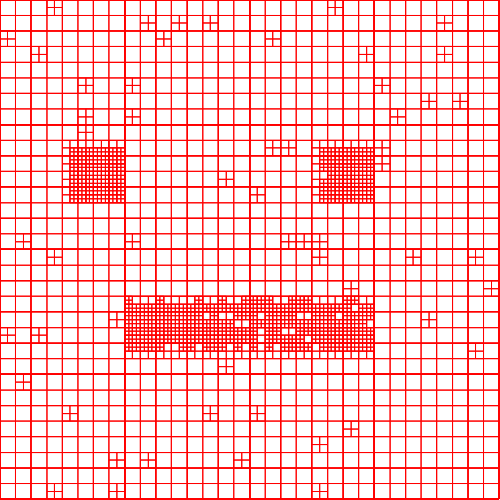
\includegraphics[scale =0.5]{lol.png}
        \end{center}
   
    \end{enumerate}
    
    
    
    
    
    
    
    
    
    
    
\section{Choix du meilleur algorithme}
\begin{center}
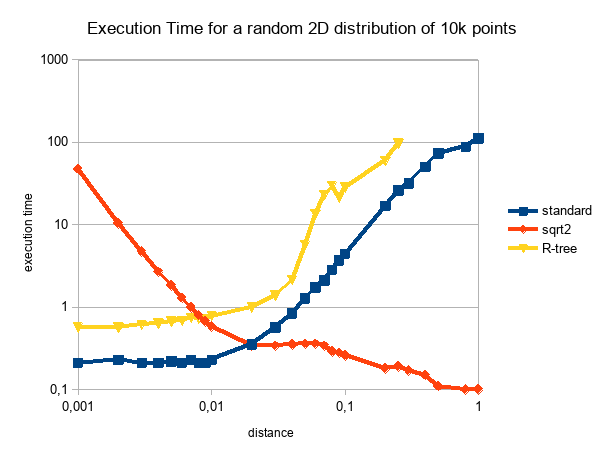
\includegraphics[scale=3]{comparaison_algos.png}
\captionof{figure}{Performances des différents algorithmes en fonction de la distance (proportionnelle à la densité à $n$ constant)}
\bigbreak
Au vu ce ces résultats, on comprend qu'il est nécessaire de programmer un 'sélecteur' qui va choisir le meilleur algorithme (et ses paramètres éventuels) en fonction de l'entrée. 
\end{center}


\clearpage
\captionof{figure}{Le schéma de fonctionnement global}
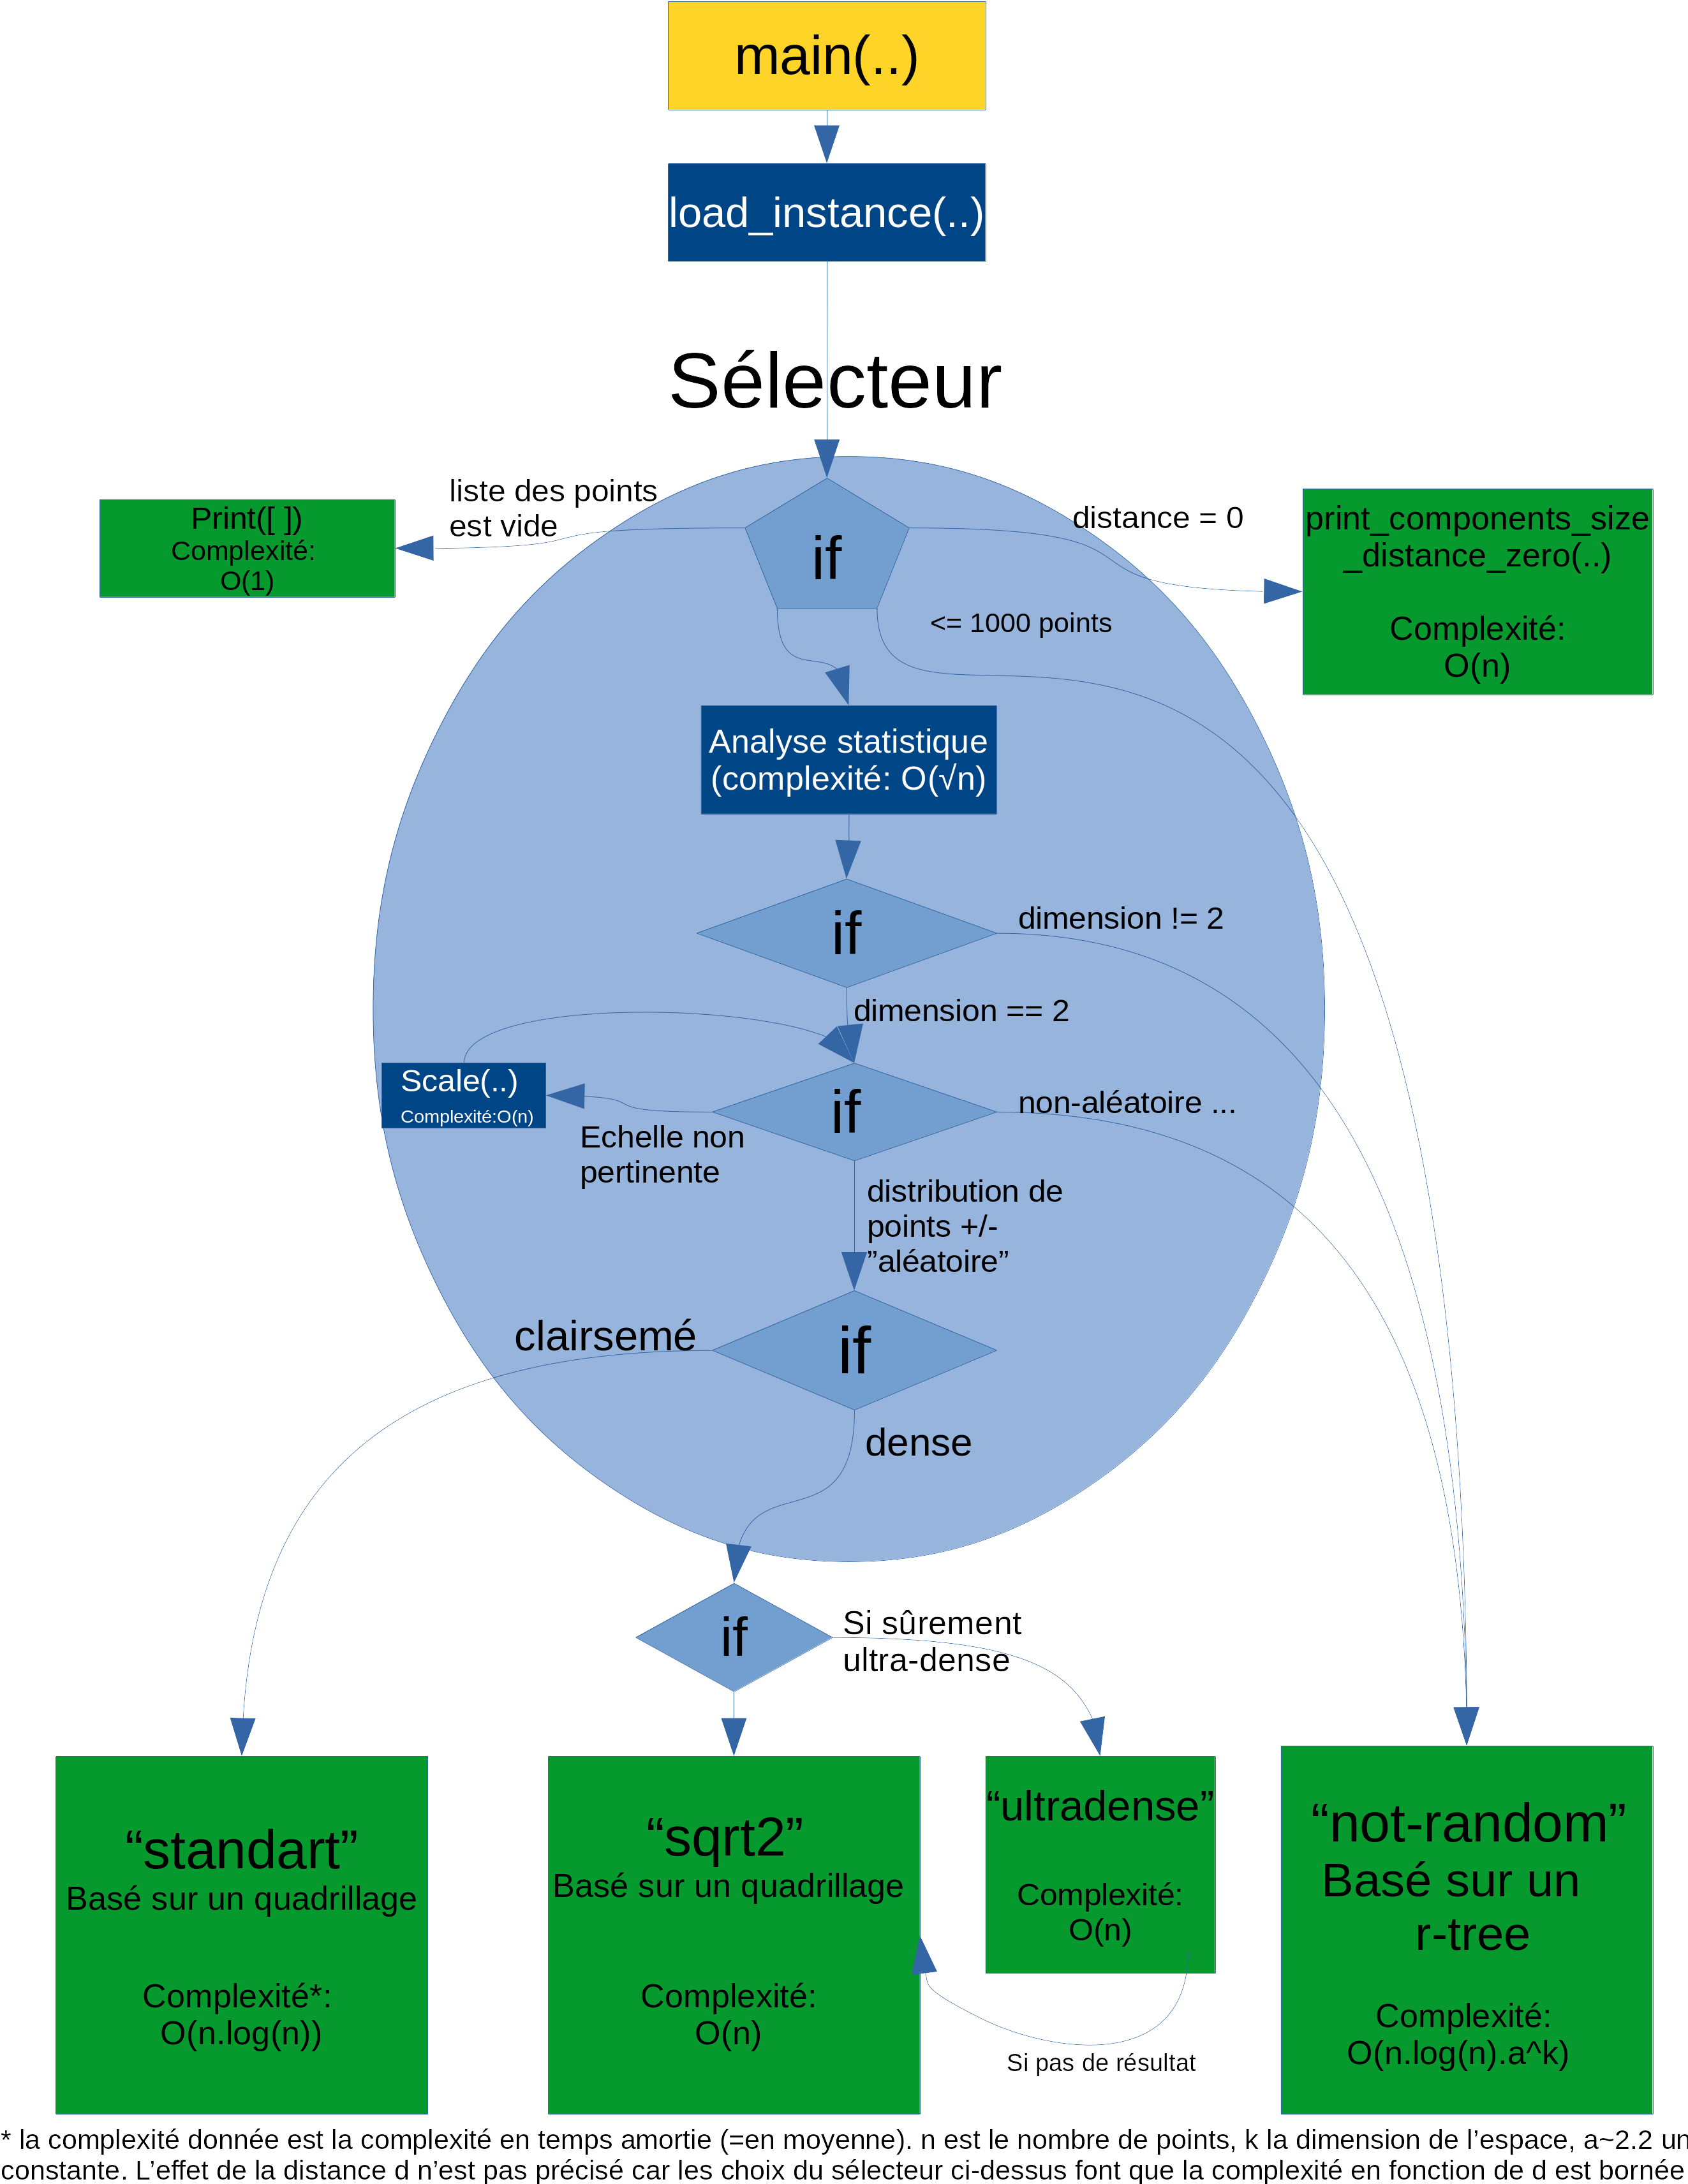
\includegraphics[scale=0.24]{fonctionnement.png}













\section{Performances}
\smallbreak 
Nota Bene: Dans cette section, on considère les performances de tous les algorithmes, intelligement choisis par le sélécteur. Le programme va choisir et exécuter l'algorithme qu'il pense être le meilleur.\\
    \begin{enumerate}
    \item \textbf{En fonction de $n$ (en dimension 2)}\\
\begin{center}
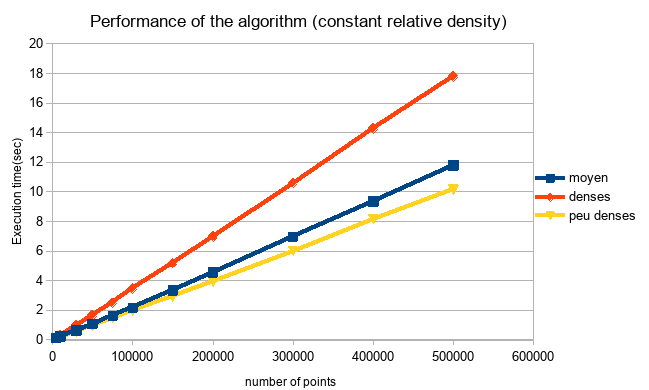
\includegraphics[scale=2.5]{perfs_densite_cste.png}
\captionof{figure}{Performances à densité constante}
\end{center}
		    On obtient ici une complexité expérimentale en $\mathcal{O}(n \log n)$ à densité constante. Le temps d'exécution dépend aussi de $d$ car cela influe sur le nombres de cases à parcourir dans le quadrillage dans le cas des 2 premiers algorithmes, mais la complexité en fonction de d est bornée. Le cas où la distribution n'est pas aléatoire est plus difficile à quantifier (quelle est la "pire" distribution?), mais lorsque l'algorithme 'not-random' est appelé on observe des performances similaires à un facteur 6 près ( environ 6x plus lent).
\clearpage
 \item \textbf{En fonction de la distance/densité (dimension 2)}\\
\begin{center}

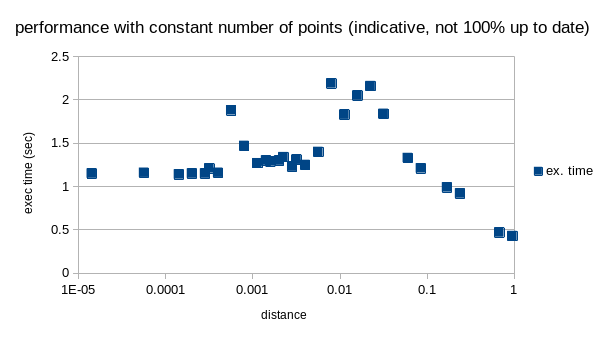
\includegraphics[scale =0.7]{perfs_with_ditance.png}
\captionof{figure}{Performances en fonction de la distance/densité}
\end{center}

On voit bien les différents niveaux où le programme modifie les paramètres/ change d'algorithme (les pics; où les performances des différents algorithmes se dégradent car on sort de leur "domaine de compétence").
De gauche à droite, une distribution peu dense avec la taille des cases forcée à $\frac{1}{\sqrt{n}}$, les distribution médianes (avec un facteur adaptatif), les distributions denses employant l'algorithme "sqrt2".
\smallbreak
Les niveaux de \textbf{densité} (constants pour toute entrée) limites sont $\frac{\pi}{24}$ et $\frac{\pi}{2}$.
\smallbreak
Les cas extrêmes sont encore améliorés dans une version plus récente de l'algorithme (voir Choix de l'algorithme).
 
\bigbreak
 \item \textbf{En fonction de la dimension}\\
\begin{center}\hspace{-6mm}
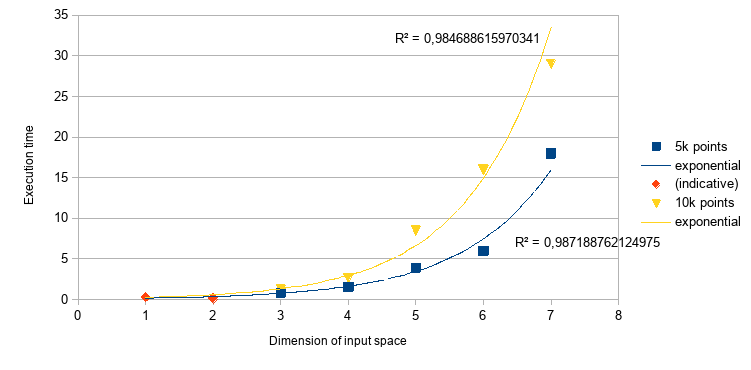
\includegraphics[scale=2.3]{perfs_dimension.png}
\captionof{figure}{Performances en fonction de la dimension, à densité constante}
\end{center}
Les valeurs pour les dimensions 1 et 2 sont indicatives pour la courbe 5k points, notamment car en dimension 2 on utilise un algorithme différent.\\
On obtient ici une complexité expérimentale exponentielle par rapport à la dimension d'entrée.

(Nota Bene: en dimension quelquonque, la densité n'est évidemment plus proportionnelle à $\frac{1}{\sqrt{n}}$, la formule exacte se situe l.42 du code dans la fonction facteur\_optimal)


















\section{Evolution du programme}
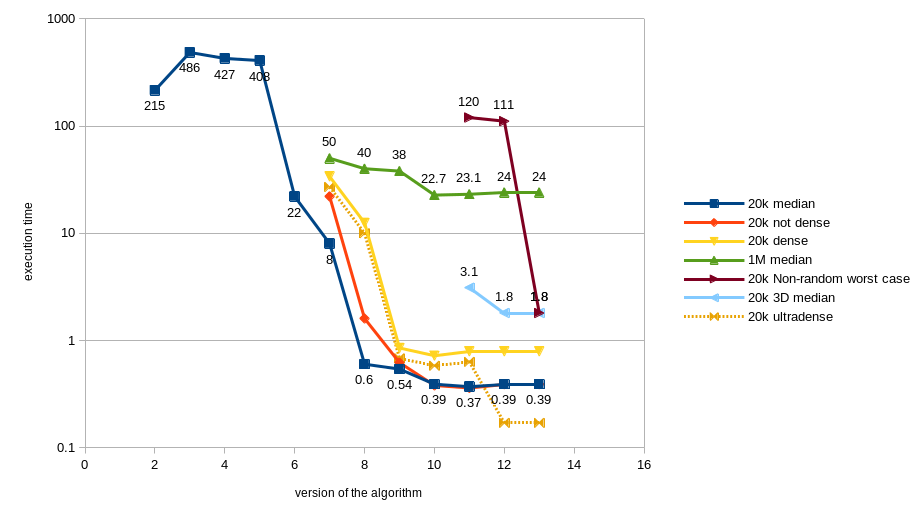
\includegraphics[scale=0.7]{perf_version_algo.png}
\captionof{figure}{Performances pour différentes entrées au fur et à mesure des avancées}
\bigbreak
Révisions majeures:\\
\begin{tabular}{ll}
   1 & ne marche pas \\
   2 &  algorithme naif, "rapide" mais oublie certaines liaisons :-|\\
   3 & algorithme naif + fusion naive mais juste\\
   6 & un (r-)arbre qui regroupe les points, on ne regarde que les voisins\\
   7 & un quadrillage à la place d'un arbre\\
   8 & la méthode de rassemblement (définitive) intelligente\\
   9 & sélection intelligente de l'algo et des paramètres\\
   10 & ne regarder qu'1/4 des cases voisines, éviter de repasser sur les mêmes couples\\
   11 & Introduction du r-tree en dimension quelquonque, optimisant aussi les distributions non-aléatoires\\
   13 & Introduction des quadrants "denses" optimisant la résolution des zones d'espaces très denses
\end{tabular}



















\section{Possibilités d'amélioration}

Nous avons l'impression d'heurter un mur pour la performance des entrées 2D aléatoires, peut-être est-ce le principe (quadrillage) qui atteint ses limites?
\smallbreak
\bigbreak
Le R-tree, bien plus sophistiqué, peut encore être soumis à de nombreuses améliorations, notamment:\\
\smallbreak
- Les quadrants feuilles denses doivent tous demander à tous s'ils sont liés. Bien que chaque appel soit en moyenne (cout amorti) rapide, le tout coûte O((nombre de quadrants denses)²) et est une cause majeure du ralentissement de l'algorithme, surtout en dimensions supérieures quand toute la distribution est dense. Il faudrait introduire un système de détection de voisins peu coûteux (compliqué en dimension quelquonque, mais faisable).
\smallbreak
- En coût mémoire: pour l'instant chaque quadrant transmet ses points intérieurs à ses enfants (ce qui est nécessaire) mais les garde en mémoire jusqu'à la fin de l'éxecution. Ces informations sont hautement inutiles et "vider" au fur et à mesure les quadrants qui ne sont pas des feuilles fera un bien fou à notre mémoire. Difficulté d'implémentation: facile.





\section{Conclusion}
C'était cool - Michaël\\
J'avoue - Clément
\bigbreak
Nota Bene: Il est possible que nous ayons répondu au problème; pour les détails techniques, voir le Résumé (1).
\end{enumerate}
\end{document}
